\section{Pulsdetektering}\label{sec_de_im_te_puls}
\textit{I dette afsnit beskrives designet, implementeringen og testen af den valgte pulssensor. Først designes opsætningen af pulssensoren og dets algoritme til det specifikke formål, hvorefter dette implementeres. Afslutningsvist bliver algoritmen vedrørende pulsdetektering testet i forhold til opstillede krav i \secref{puls_krav_}}.

\subsection{Design} \label{sec_design_puls}
Pulssensoren skal benyttes til at beskrive intensiteten af aktiviteten, som er beskrevet i \secref{subsub:ak_int}. Heraf kan effekten af aktiviteten bestemmes, hvilket vil blive afspejlet som en motiverende faktor i forbindelse med visualisering i GUI. \newline
Pulssensoren SEN-11574 er valgt til dette projekt, da den er en optisk pulssensor og er derfor mere sikker for brugeren, som beskrevet i \secref{sec:pulssensor}. Ydermere er en optisk sensor alsidig i forhold til placering, idet denne type sensor blot kræver en placering over en arterie for at kunne måle pulsen. SEN-11574 kræver en spændingstilkobling på 3~V til 5~V for at være funktionel og forbruger 4~mA ved en forsyning på 5~V. På sensorens printplade findes et aktivt filter\fxnote{Et aktivt filter er en type af analog elektronisk filter, der anvender aktive bestanddele, såsom en forstærker.} samt en forstærker, som tilsammen øger amplituden for pulsbølgen og normaliserer signalet omkring et referencepunkt, hvilket fjerner DC spænding i signalet. \citep{Murphy2016,Murphy2016_sensor}\\
Pulssensoren designes således, at pulsen (BPM) beregnes for brugeren i GAP peripheral og sendes til GAP central, hvilket fremgår af \figref{fig:puls_pseudo}.
\begin{figure}[H]
	\centering
	\includegraphics[scale=0.5]{figures/cDesign/puls_pseudo.png}
	\caption{På figuren ses et flowchart over algoritmen vedrørende detektering af BPM under alle aktiviteterne. Pulssensorens algoritme skal registrere tre pulsslag førend pulsen kan beregnes ud fra disse værdier.}
	\label{fig:puls_pseudo}
\end{figure}
Ovenstående figur repræsenterer algoritmen vedrørende detektering af BPM. Pulssensoren opfanger pulssignalet fra brugerens øreflip, hvorefter dette signal bliver signalbehandlet førend detektering af pulsslag startes. Der ønskes at detektere pulsen ved at beregne varigheden mellem tre pulsslag med udgangspunkt i det systoliske peak, hvilket fremgår af \secref{sec:pulssensor}. Dette peak har større amplitude end peaket for diastole, hvormed signalbehandlingen skal forstærke det systoliske peak og dæmpe det diastoliske peak.  \\
Dataet fra pulssensoreren signalbehandles i form af en division og kvadrering. Dette vil medføre, at det største peak i signalet vil blive forøget i amplitude, og de mindre peaks vil opnå en lavere amplitude, hvilket ses på \figref{fig:behandlet_puls}. 
\begin{figure}[H]
	\centering
	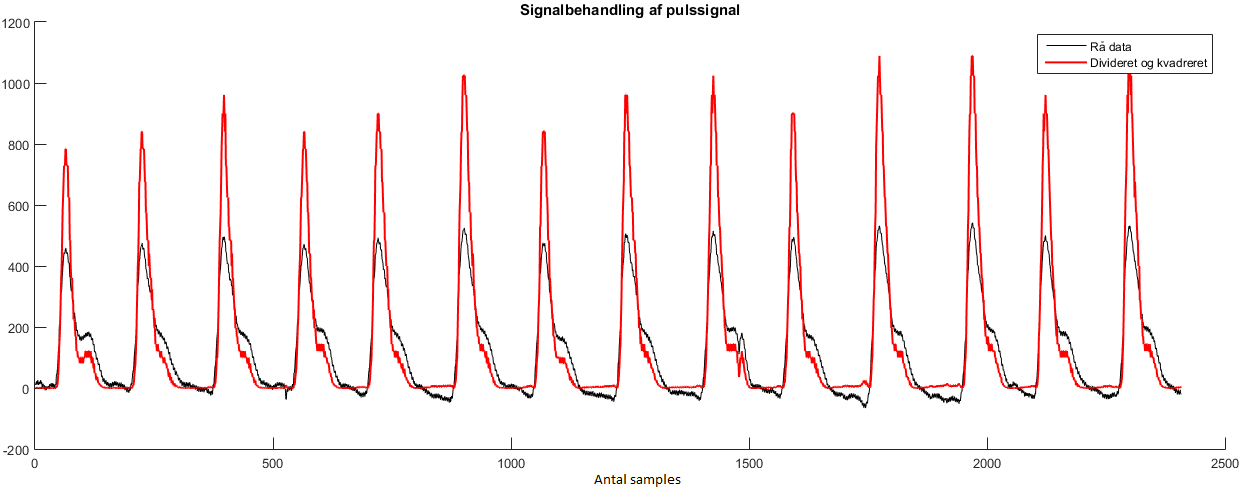
\includegraphics[scale=0.4]{figures/cDesign/puls_ore_behandlet.png}
	\caption{På figuren ses algoritmens signalbehandling af et råt pulssignal. Den sorte kurve er det rå pulssignal, og den røde kurve er det dividerede og kvadrerede signal.}
	\label{fig:behandlet_puls}
\end{figure}
Som resultat af signalbehandlingen på \figref{fig:behandlet_puls} ses det, at amplituden på det behandlede signal er forøget, hvorimod de mindre peaks er formindsket. De største peaks i signalet repræsenterer den systoliske periode i hjertecyklussen, hvilket er det peak, der benyttes til at bestemmes BPM for signalet. For at kunne bestemme BPM for signalet, bliver der implementeret en tærskelværdi. Denne værdi skal signalet overskride for at kunne blive detekteret som et systolisk peak. Tærskelværdien for algoritmen bestemmes med udgangspunkt i en pulsmåling, hvor sensoren er placeret på øreflippen. Dette fremgår af \figref{fig:taerskel_puls}.
\begin{figure}[H]
	\centering
	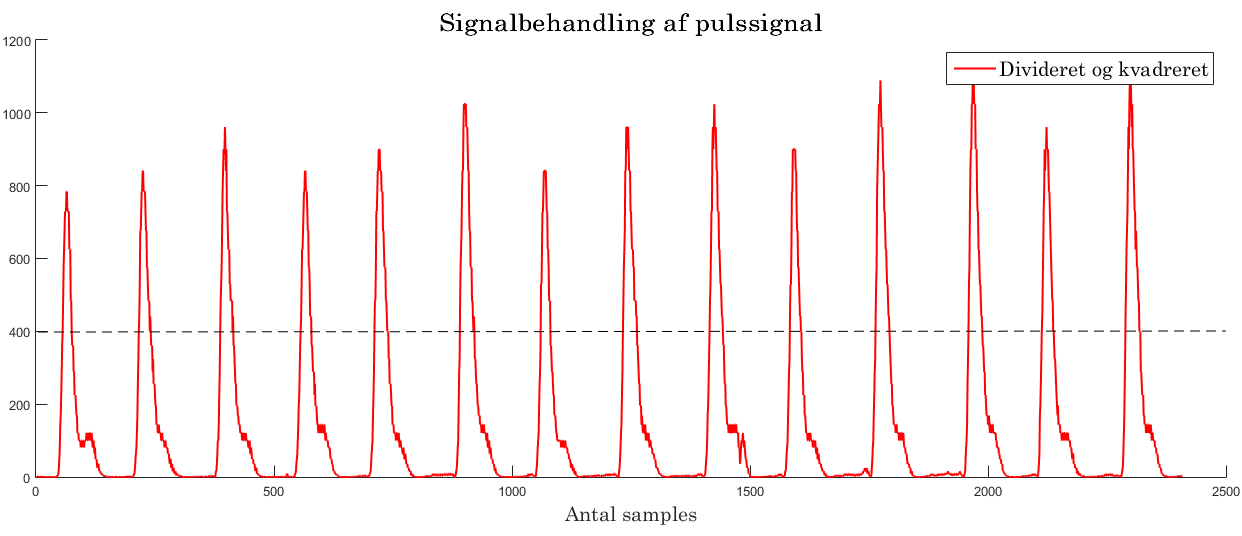
\includegraphics[scale=0.4]{figures/cDesign/puls_taerskel.png}
	\caption{På figuren ses en pulsmåling foretaget på øreflippen. Den røde kurve er en signalbehandlet pulsmåling fra øreflippen, og den sorte stiplede linje er algoritmens tærskelværdi, som har en værdi 400.}
	\label{fig:taerskel_puls}
\end{figure} \vspace{-0.5cm}
Det behandlede signal fremgår af figuren, hvortil der er indtegnet en tærskelværdi, som alle de systoliske peaks vil overskride. Denne tærskelværdi vil medføre, at det systoliske tryk overstiger tærskelværdien, hvortil det diastoliste tryk vil befinder sig under. Algoritmen vil benytte varigheden mellem de forekomne systoliske tryk til at kunne beregne BPM med udgangspunkt i tre detekterede peaks. 

\subsection{Implementering} \label{puls_impl}
Pulssensoren har 3 pins til henholdsvis spændingsforsyning, ground og outputsignal. Disse pins kobles til hver sin pin på GAP peripheral. Outputsignalets pin skal designes i PSoC Creator, således MCUen modtager pulssensorens signaler fra den pågældende pin. Dette gøres ved at indsætte henholdsvis en UART serie kommunikationsblok (SCB) og SAR ADC i topdesignet. UARTen bruges til, at sensoren og MCUen kan kommunikere med hinanden. Standardindstillingerne for denne blok benyttes til konfigurationen af MCUen. \newline
Outputsignalet fra sensoren er et analogt signal, hvormed dette signal opsamles af en ADC for at skabe en konvertering til et digitalt signal. ADCens design skal derfor konfigureres således, at denne bearbejder én single ended kanalinput fra pulssensoren. Yderligere indstilles samplingsfrekvensen for ADcen for den pågældende inputkanal til 35~Hz, med henhold til \secref{krav_adc}. \\
Efter konfigurering af UART og ADC i topdesignet, skal de korrekte pins indstilles i pinopsætning. UART tildeles interne RX-, og TX-pins, hvorimod ADCens inputpin skal indstilles til den pin, som outputtet fra sensoren er placeret i, hvilket er valgt til pin 2.0. 
\begin{figure}[H]
	\centering
	\includegraphics[scale=0.4]{figures/cDesign/Puls_ckode.png}
	\caption{På figuren ses pulssensorens algoritme i C kode beskrevet med pseudokode.}
	\label{fig:puls_pseudo_c}
\end{figure} \vspace{-0.5cm}
Første trin, efter dataopsamlingen fra pulssensoren, er en konvertering af det analoge signal til et digitalt. Derefter undersøges det, hvorvidt det konverterede data er klar, hvilket der benyttes en indbygget kodegenerering til. Hvis data er klar, da starter algoritmens time counter som starter optælling af samples. Når en sample er klar, bliver den kvadreret og divideret, som det beskrives i \secref{sec_design_puls}. Den behandlede sample gemmes i en variabel, 'Value[0]'. Når der kommer en ny sample, vil den forrige sample blive gemt i en ny variabel, 'Value[1]', og den nye sample gemmes i den anden variabel. \\
Yderligere tæller algoritmen antallet af pulsslag, ved at vurdere om 'Value[0]' er under tærkselværdien og 'Value[1]' er over. Hvis dette er tilfældet, vil der blive lagt én til antal pulsslag, dog maksimalt til antal pulsslag er <4. Algoritmen erydermere designet således, at at den registrerer et pulsslag, når en tidligere sample er over tærskelværdien og den efterfølgende sample er under. Derfor vil algoritmen kunne beregne BPM for brugeren, med det forbehold, at antallet af pulsslag skal være 3. Time counteren benyttes i denne forbindelse, til at optælle antallet af samples mellem 3 pulsslag. Beregningen foretages ved at bestemme den gennemsnitlige varighed mellem 3 pulsslag, for derefter at dividere 60 sekunder med den gennemsnitlige varighed. Når beregningen er foretaget, vil BPM for brugeren blive sendt til GAP central gennem bluetooth, hvorefter algoritmens værdier nulstilles.


\subsection{Test}
Pulssensoren testes, for at undersøge hvorvidt den designede og implementerede algoritme kan bestemme den rigtige BPM ved et simuleret signal. Ydermere testes sensoren og algoritmen, ved at benytte Vernier, Excercise Heart Rate Monitor, som reference for den BPM som pulssensoren og den tilhørende algoritme bør sende via bluetooth. \\
Testen udføres med henhold til de opstillede krav og tilhørende tilladte afvigelser opstillet i \secref{puls_krav}.

Algoritmens funktionalitet testes ved at indsende et simuleret signal, som består af et absolut sinussignal. Peaks på dette simulerede signal skal repræsentere de systoliske peaks i en pulssignal optages med en pulssensor.\\
Det simulerede signal sendes ind i MCUen, hvorefter det undersøges hvorvidt time counteren detekterer varigheden mellem overskridelser af algoritmens opsætning. Når pulsen er bestemt, benyttes programmet Real Term til at printe algoritmens slutresultat, som er BPM. \\
Det indsendte signal er et absolut sinussignal, som har en frekvens på 0,6~Hz og en samplingsfrekvens på 188~Hz. Ydermere er det array, som indsendes til MCUen, på 1451 samples. Derfor kan det bestemmes hvilken puls, som algoritmen bør printe i Real Term. \\
Der indsendes 1451 samples og benyttes en samplingsfrekvens på 188~Hz, hvormed arrayet har en længde på 7,7 sekunder. Idet der er tale om et absolut sinussignal på 0,6~Hz, vil der opstå 9,26 peaks i det indsendte signal. Dette vil betyde, at algoritmen skal udregne og printe tre værdier for pulsen, idet der er 9 fuldstændige peaks. \\
Når der er 9,26 peaks og arrayet har en varighed af 7,7 sekunder, vil der være 0,83 sekunder mellem hver overskridelse af tærskelværdien. Pulsen bestemmes, som det fremgår af \eqref{eq:puls_teori}.
\begin{equation}
\frac{60~sekunder}{Varighed~mellem~samples} = \frac{60~sekunder}{0,83~sekunder} = 72~BPM
\label{eq:puls_teori}
\end{equation} 
Derfor vil det indsendte signal medføre en værdi af 72 BPM. Det er forventeligt, at algoritmen vil beregne og printe en puls, som har en værdi af 72 BPM.

Algoritmen er bestemt til at nulstille sin time counter hver gang der registreres tre tilfælde, hvor en sample er gået under tærskelværdien. Derfor vil algoritmen gøre brug af time counterens optalte antal samples til at bestemme pulsen for den pågældende periode. \\
Ved at indsende det simulerede signal fremgår det af \figref{fig:timecounter_puls_realterm}, hvordan time counteren nulstilles, når der er registreret tre tilfælde. Ydermere ses det i \tabref{tab:test_puls_realterm}, at Real Term har printer de forventede værdi for BPM.
\begin{figure}[H]
	\centering
	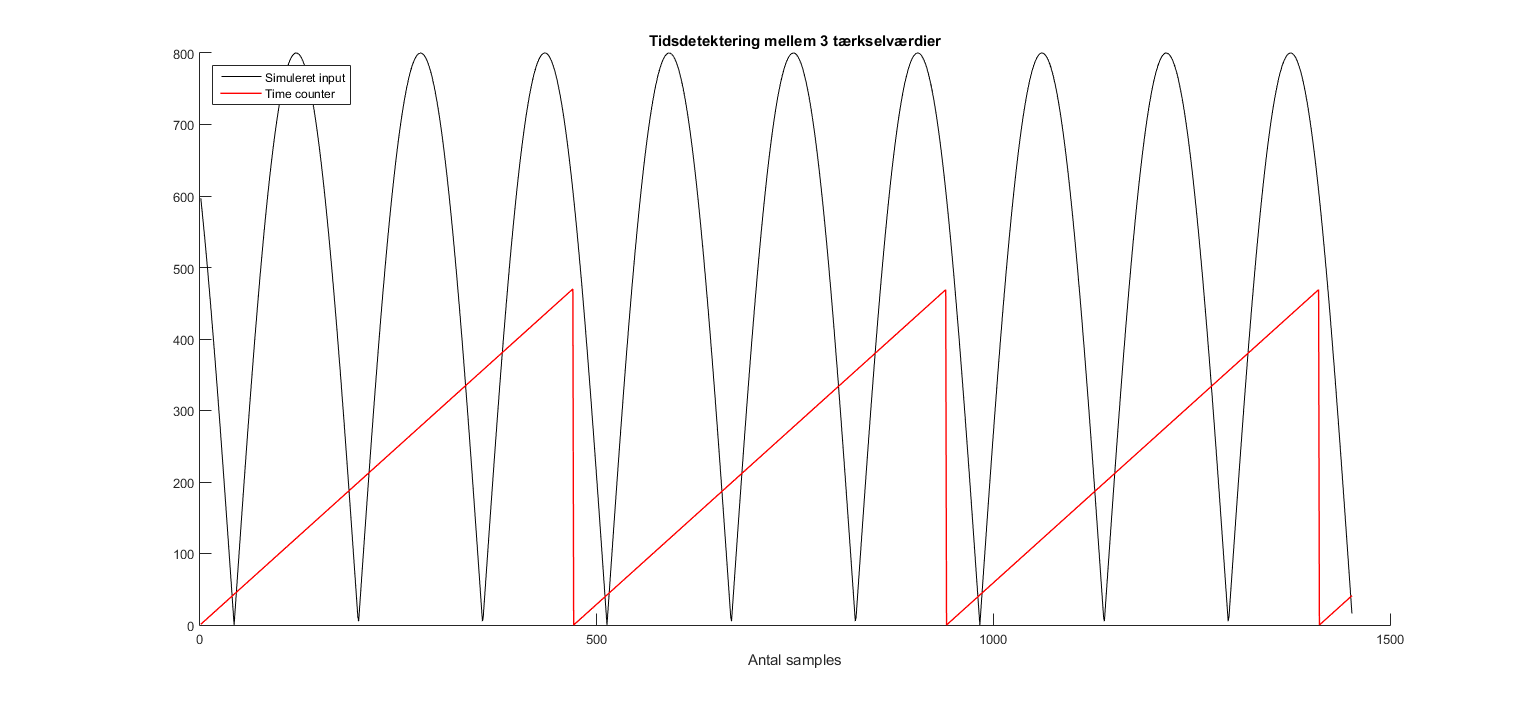
\includegraphics[scale=0.4]{figures/cDesign/timecounter_puls_pic.png}
	\caption{På figuren ses algoritmens timecounter, som tæller op, indtil en sample på det tredje pulsslag er gået under tærskelværdien. Efterfulgt af dette vil time counteren nulstilles og starter samme procedure.}
\label{fig:timecounter_puls_realterm}
\end{figure}
\begin{table}[H]
	\centering
	\begin{tabular}{ccc}
		\hline
		\rowcolor[HTML]{C0C0C0} 
		Forventet værdi [BPM] & Modtaget værdi [BPM] & Afvigelse [\%]\\ \hline
		72 - 72 - 72          & 72 - 72 - 72         & 0 - 0 - 0 \\ \hline
	\end{tabular}
	\caption{I tabellen ses resultaterne fra algoritmens beregning af pulsen på et simuleret inputsignal. Tabellens kolonne; Modtaget værdi, er resultatet fra Real Term.}
	\label{tab:test_puls_realterm}
\end{table} \vspace{-0.5cm}

Det fremgår af \figref{fig:timecounter_puls_realterm}, at algoritmen tæller indtil tre peaks er detekteret. Herefter beregner algoritmen pulsen ud fra det antal samples, som findes inden for disse tre peaksdetekteringer. Herefter printes pulsen i Realterm, hvor værdierne er illustreret i tabellen. Det fremgår ydermere, at de modtagede værdier har 0\% afvigelse fra de forventede værdier. \\
Det kan derfor konkluderes, at pulssensoren og den tilhørende algoritme fungerer som tiltænkt ved benyttelse af et simuleret inputsignal. 

Der foretages yderligere en test, med henblik på at vurdere hvorvidt pulssensoren opfylder de opstillede krav i \secref{puls_krav}. \\
Pulssensoren og den tilhørende algoritme testes på en person ved en stillesiddende aktivitet, hvoraf personens BPM forventes dermed at være stabil. Yderligere vil der blive benyttet en pulsmåler i form af Vernier, Excercise Heart Rate Monitor, som benyttes som reference for den beregnede BPM af algoritmen. Denne pulssensors data vil blive printet i programmet Logger Pro, og systemets BPM vil blive printet i Realterm. \\
Resultaterne af den udførte test fremgår af \tabref{tab:test_pulssystem}.
\begin{table}[H]
	\centering
	\begin{tabular}{ccc} \hline
		\rowcolor[HTML]{C0C0C0} 
			Gennemsnitlig puls LoggerPro {[}BPM{]} & Gennemsnitlig puls Algortime {[}BPM{]} & Afvigelse {[}\%{]} \\ \hline
			60,4 & 64,5 & 6,4 \\ \hline
		\end{tabular}%
	\caption{I tabellen ses det den gennemsnitlige puls fra Logger Pro og Real Term. Det fremgår, at pulssensoren og den tilhørende algoritme har en afvigelse på 6,4\%.}
	\label{tab:test_pulssystem}
\end{table} \vspace{-0.5cm}
Det fremgår i \tabref{tab:test_pulssystem}, at testen af pulssensoren og den tilhørende algoritme viser en gennemsnitlig afvigelse fra referenceværdien på 6,4\%. Dermed overholder pulssensoren de opstillede krav i \secref{puls_krav}.